\documentclass[journal]{IEEEtran}

% ---------- Packages ----------
\usepackage{amsmath,amssymb}
\usepackage{graphicx}
\usepackage{booktabs}
\usepackage{multirow}
\usepackage{array}
\usepackage{textcomp}
\usepackage{url}

\hyphenation{ap-pli-cant ap-pli-cants cali-bra-tion cali-brator
  dis-cri-mi-na-tion frag-ile iso-tonic oscil-la-tion pertur-ba-tion
  pertur-ba-tions prob-abil-ity recal-li-brate re-sam-pling ro-bust-ness
  sen-si-tive super-vised thresh-old un-cal-i-brat-ed}

\title{Stability-Aware and Confidence-Guided Explainable AI for
Credit Risk Assessment: An Audit Layer with Explanation-Reliability
Routing}

\author{
\IEEEauthorblockN{Jatin Sachdeva, Siddharth Singh, Gauravi Singh, and Anshika Rai}
\IEEEauthorblockA{\textit{Department of Computer Science and Engineering}\\
\textit{Kalinga Institute of Industrial Technology}\\
Bhubaneswar, India}
}

\begin{document}
\maketitle

\begin{abstract}
Machine-learning scorecards inform lending decisions, yet discrimination alone
does not make a model auditable: probabilities may be miscalibrated, and local
explanations may shift under measurement noise. We describe an audit
layer---not a replacement predictor---over gradient-boosted classifiers that
reports three reliability signals per applicant: a calibrated default risk, a
per-case explanation-stability score $S(x)$ under bounded perturbations, and a
top-$k$ SHAP--LIME agreement index. These signals, together with the decision
margin and a split-conformal $p$-value, drive human-review routing. Under a
leakage-free protocol on German Credit and Australian Credit Approval,
SMOTE-ENN raised minority recall while degrading AUC and Brier score; isotonic
calibration cut expected calibration error by 56\% (0.136 to 0.060) and 38\%
(0.106 to 0.066). On German Credit, 16.7\% of test cases carried unstable
explanations ($S<0.8$), nearly independent of the decision margin
($\rho_s=0.042$), so margin-based abstention cannot surface them. At 55\%
matched coverage, adding the stability rule reduced the composite review-need
rate among automatically decided applications from 0.282 to 0.209---a gain we
show to be partly definitional. Mean top-5 SHAP--LIME Jaccard agreement was
0.353 on German Credit and 0.498 on Australian Credit. We also measure cost:
prediction takes about 0.15~ms/case, the stability audit 32--39~ms/case, and
the SHAP--LIME audit 279--445~ms/case, so the explanation audit is a batch-time
cost rather than a few milliseconds of online latency.
\end{abstract}

\begin{IEEEkeywords}
credit risk, explainable artificial intelligence, explanation stability,
probability calibration, SHAP, LIME, selective prediction, conformal
prediction, class imbalance
\end{IEEEkeywords}

\section{Introduction}

Credit risk assessment estimates how likely a borrower is to fail on a
repayment obligation. Lenders consume such estimates when approving or
declining an application, when deciding which additional checks to commission,
and when sizing portfolio exposure. Machine-learning models capture
interactions among applicant attributes that linear scorecards miss, but
deploying them in consequential decisions raises three linked difficulties:
class imbalance, the reliability of the emitted probabilities, and the
trustworthiness of the explanations offered alongside each decision.

Class imbalance arises when one outcome is markedly rarer than the other. A
model trained on skewed data can post high accuracy while recovering few
defaulters. Resampling remedies such as SMOTE~\cite{chawla2002smote} and SMOTE
combined with Edited Nearest Neighbours (SMOTE-ENN)~\cite{batista2004study}
are widely adopted, yet resampling must remain confined to training folds;
otherwise information from validation or test observations leaks into
synthetic samples and inflates measured performance.

Probability reliability is a second concern. A score of 0.70 invites the
reading ``a 70\% chance of default'', and that reading is warranted only when
the probabilities are calibrated~\cite{guo2017calibration}. Explanation
stability is a third. SHAP~\cite{lundberg2017unified} and LIME~\cite{ribeiro2016why}
nominate the influential attributes behind an individual prediction, yet those
nominations can move under small input changes~\cite{alvarezmelis2018robustness,
ghorbani2019interpretation}, and the two methods may disagree on the same
applicant~\cite{krishna2022disagreement}.

Recent credit-scoring studies have advanced these axes largely one at a time:
ensembles with SMOTE-ENN~\cite{aruleba2024credit,aruleba2025improved},
comparisons of boosting families~\cite{nguyen2025comparative}, generative
oversampling~\cite{kwon2026generative}, focal-loss networks~\cite{chab2026csanet},
SHAP rank stability under resampling~\cite{shawabkeh2026explainable},
SHAP-driven calibrated ensembles~\cite{japinye2025explainable}, and qualitative
arguments that imbalance erodes explanation trust~\cite{tufail2026signal}. As
far as we can establish, no prior study couples calibrated risk, per-case
explanation stability under plausibility-preserving perturbations, and
cross-method agreement inside an explicit human-review policy, and none asks
whether explanation instability is visible from the decision margin. Closing
that gap is the purpose of this paper.

\emph{Contributions.}
\begin{enumerate}
\item A per-case stability score. We define $S(x)$, a rank-correlation measure
computed over bounded perturbations of noise-susceptible numeric attributes,
together with a top-$m$ set-overlap variant.
\item Evidence that margin and explanation reliability are complementary. On
German Credit, explanation instability is nearly uncorrelated with the
decision margin ($\rho_s=0.042$) and affects 16.7\% of test cases; flagged
applications are not more error-prone than unflagged ones (error 0.280 versus
0.297).
\item A reliability audit layer. Calibration (Platt and isotonic), SHAP--LIME
agreement, and $S(x)$ are combined with a conformal $p$-value into a single
routing rule, assessed at matched coverage, with an explicit account of which
gains hold by construction.
\item A leakage-free evaluation of class weighting, SMOTE, and SMOTE-ENN across
XGBoost, LightGBM, and CatBoost on two public datasets, supplemented by a
group-wise behaviour check and a measured overhead breakdown.
\end{enumerate}
Section~\ref{sec:related} reviews related work, Section~\ref{sec:framework}
presents the framework, Section~\ref{sec:setup} the experimental protocol,
Section~\ref{sec:results} the results, Section~\ref{sec:threats} the threats to
validity, and Section~\ref{sec:conclusion} concludes.

\section{Related Work}
\label{sec:related}

\subsection{Class Imbalance in Credit Risk}
SMOTE~\cite{chawla2002smote} synthesises minority examples by interpolation;
hybrids such as SMOTE-ENN clean overlapping regions of class space~\cite{batista2004study};
and the broader repertoire is surveyed in~\cite{he2009learning}. Within credit
risk, Aruleba and Sun coupled ensembles with SMOTE-ENN and model
explanations~\cite{aruleba2024credit} and subsequently proposed a stacked
ensemble with hybrid resampling~\cite{aruleba2025improved}. Nguyen and Ngo
benchmarked boosting algorithms for personal default prediction~\cite{nguyen2025comparative};
Kwon evaluated generative oversampling against SMOTE variants~\cite{kwon2026generative};
and Chab and Jeon introduced a type-aware dual-tower network with focal
loss~\cite{chab2026csanet}, noting that focal loss can be poorly calibrated.
These studies optimise discrimination. None reports the calibration of the
resulting probabilities, or the effect of imbalance handling on explanation
stability---the latter raised qualitatively by Tufail and Sohail~\cite{tufail2026signal}.

\subsection{Explainability in Credit Risk}
SHAP~\cite{lundberg2017unified} supplies Shapley-value attributions and
LIME~\cite{ribeiro2016why} builds local surrogates. Misheva et al.\ applied
both to credit risk~\cite{misheva2021explainable}; Shawabkeh et al.\ audited
SHAP rank stability under bootstrap resampling~\cite{shawabkeh2026explainable};
Xin used counterfactual explanations for fair scoring on German
Credit~\cite{xin2026explainable}; and Japinye and Adedugbe combined calibrated
ensembles with SHAP while examining temporal explanation
stability~\cite{japinye2025explainable}. These analyses address global
attribution stability, model-level calibration, or recourse. General-purpose
work establishes that interpretations are fragile~\cite{alvarezmelis2018robustness,
ghorbani2019interpretation} and that methods disagree~\cite{krishna2022disagreement},
but per-case local stability has not been embedded in a credit decision pipeline.

\subsection{Calibration, Uncertainty, and Selective Prediction}
Platt scaling~\cite{platt1999probabilistic} and isotonic
regression~\cite{zadrozny2002transforming,niculescu2005predicting} correct
probability estimates, while Guo et al.\ popularised the expected calibration
error~\cite{guo2017calibration}. Selective prediction with a reject
option~\cite{geifman2017selective} trades coverage against risk, and conformal
prediction delivers distribution-free uncertainty with finite-sample
guarantees~\cite{angelopoulos2023conformal,vovk2005algorithmic}. Marjanovi\'c
et al.\ showed that model instability propagates into explanations and
uncertainty estimates in NLP~\cite{marjanovic2024investigating}.

\subsection{Positioning}
Table~\ref{tab:related} summarises coverage. The closest studies are~\cite{tufail2026signal}
(imbalance and explanation trust) and~\cite{shawabkeh2026explainable} (SHAP
stability). Neither converts explanation quality into an operational review
policy. Our uncertainty component is a conformal $p$-value: it is implemented,
but it is inactive on the datasets studied (Section~\ref{sec:routing}), so we
mark it partial.

\begin{table}[t]
\caption{Coverage of Recent Work ($\checkmark$ = addressed; $\circ$ = partial;
$-$ = absent).}
\label{tab:related}
\centering
\footnotesize
\begin{tabular}{@{}lccccc@{}}
\toprule
Study & Imbal. & Calib. & Expl.\ stab. & Uncert. & Routing \\
\midrule
Aruleba \& Sun '24~\cite{aruleba2024credit} & $\checkmark$ & $-$ & $\circ$ & $-$ & $-$ \\
Aruleba \& Sun '25~\cite{aruleba2025improved} & $\checkmark$ & $-$ & $-$ & $-$ & $-$ \\
Nguyen \& Ngo '25~\cite{nguyen2025comparative} & $\checkmark$ & $-$ & $-$ & $-$ & $-$ \\
Kwon '26~\cite{kwon2026generative} & $\checkmark$ & $-$ & $-$ & $-$ & $-$ \\
Chab \& Jeon '26~\cite{chab2026csanet} & $\checkmark$ & $\circ$ & $-$ & $-$ & $-$ \\
Tufail \& Sohail '26~\cite{tufail2026signal} & $\checkmark$ & $-$ & $\circ$ & $-$ & $-$ \\
Shawabkeh et al.\ '26~\cite{shawabkeh2026explainable} & $-$ & $-$ & $\checkmark$ & $-$ & $-$ \\
Xin '26~\cite{xin2026explainable} & $-$ & $-$ & $\circ$ & $-$ & $-$ \\
Japinye \& Adedugbe '25~\cite{japinye2025explainable} & $-$ & $\checkmark$ & $\circ$ & $-$ & $-$ \\
Marjanovi\'c et al.\ '24~\cite{marjanovic2024investigating} & $-$ & $-$ & $\circ$ & $\checkmark$ & $-$ \\
\hline
This work & $\checkmark$ & $\checkmark$ & $\checkmark$ & $\circ$ & $\checkmark$ \\
\bottomrule
\end{tabular}
\end{table}

\section{Proposed Audit Framework}
\label{sec:framework}

Figure~\ref{fig:pipeline} shows the six-stage pipeline. Stages 1--3 build and
calibrate the predictor; stages 4--6 conduct the explanation audit and convert
its output into a routing decision.

\begin{figure*}[t]
\centering
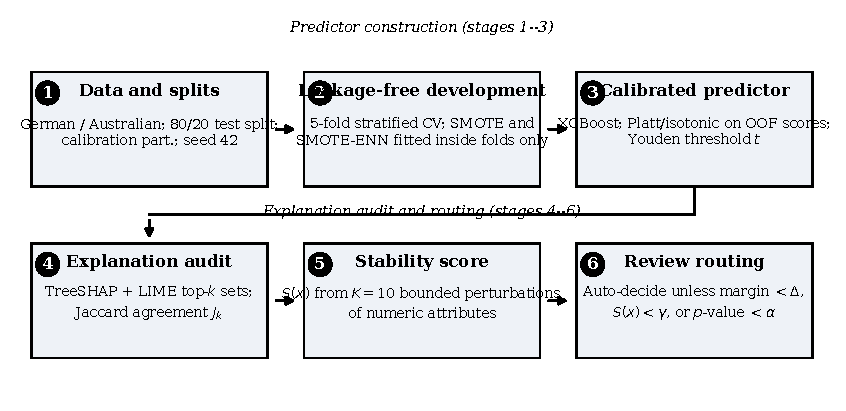
\includegraphics[width=\textwidth]{figures/fig1_pipeline.pdf}
\caption{Stability-aware, confidence-guided audit pipeline. Stages 1--3
construct and calibrate the predictor; stages 4--6 construct the explanation
audit and convert it into a review decision. Resampling is fitted inside
training folds only, calibration uses out-of-fold scores, and routing combines
the decision margin, a split-conformal $p$-value, and the stability score
$S(x)$.}
\label{fig:pipeline}
\end{figure*}

\subsection{Leakage-Free Model Development}
All resampling (SMOTE, SMOTE-ENN) is fitted inside training folds only, through
an imbalanced-learn pipeline; class weighting uses $w=n^-/n^+$ computed on each
training fold. Five-fold stratified cross-validation (CV) governs model and
strategy selection.

\subsection{Probability Calibration}
Platt (sigmoid) scaling~\cite{platt1999probabilistic} and isotonic
regression~\cite{zadrozny2002transforming} are fitted on out-of-fold
predictions within the training partition. The calibrator is chosen by
out-of-fold Brier score, with expected calibration error as a tie-breaker; the
ECE~(\ref{eq:ece}) is
\begin{equation}
\mathrm{ECE}=\sum_{b=1}^{B}\frac{|G_b|}{n}\,
  \left|\bar{p}_b-\bar{y}_b\right|,
\label{eq:ece}
\end{equation}
where $G_b$ is the $b$-th of $B=10$ equal-width probability bins, $\bar{p}_b$
the mean predicted probability in that bin, and $\bar{y}_b$ the observed
default rate. Because selection uses development data, the held-out test table
may rank candidates differently; we report both.

\subsection{Explanation Generation and Agreement}
For tree ensembles, TreeSHAP~\cite{lundberg2020local} yields exact local
attributions $\phi_j(x)$. LIME~\cite{ribeiro2016why} supplies a complementary
surrogate. For every case we record the top-$k$ feature sets of both methods,
$T^{\mathrm{SHAP}}_k(x)$ and $T^{\mathrm{LIME}}_k(x)$, and their Jaccard
agreement~(\ref{eq:jaccard})
\begin{equation}
J_k(x)=\frac{\left|T^{\mathrm{SHAP}}_k(x)\cap T^{\mathrm{LIME}}_k(x)\right|}
             {\left|T^{\mathrm{SHAP}}_k(x)\cup T^{\mathrm{LIME}}_k(x)\right|},
\label{eq:jaccard}
\end{equation}
which serves as a cross-method audit of the explanation itself.

\subsection{Explanation Stability}
For each test case $x$ we draw $K=10$ perturbations $x^{(k)}$ by jittering only
noise-susceptible numeric attributes (loan duration, amount, installment rate,
residence tenure, age, credit count, dependents) by up to $\pm 5\%$ of their
range and clipping to the empirical 5--95\% quantile envelope. These
perturbations represent reporting and measurement noise in applicant data
rather than actions an applicant could take; attributes such as age are
therefore perturbed as recorded values, not as mutable quantities. The
stability score~(\ref{eq:stability}) is
\begin{equation}
S(x)=\frac{1}{K}\sum_{k=1}^{K}\rho_s\!\left(|\phi(x)|,
  \left|\phi(x^{(k)})\right|\right),
\label{eq:stability}
\end{equation}
where $\rho_s$ is the Spearman rank correlation of absolute attributions.
Because a rank correlation computed over all attributes is dominated by noise
among near-zero attributions, we also report a top-$m$ variant~(\ref{eq:topm}),
\begin{equation}
S_m(x)=\frac{1}{K}\sum_{k=1}^{K}
  \frac{\left|T_m(x)\cap T_m(x^{(k)})\right|}
       {\left|T_m(x)\cup T_m(x^{(k)})\right|},
\label{eq:topm}
\end{equation}
with $T_m(\cdot)$ denoting the $m$ attributes of largest $|\phi|$, alongside
the normalised $\ell_1$ displacement
$\|\phi(x)-\phi(x^{(k)})\|_1/\|\phi(x)\|_1$ as a secondary measure.

\subsection{Reliability-Guided Routing}
A decision threshold $t$ is chosen on out-of-fold predictions by Youden's
$J$~\cite{youden1950index}. A case is routed to human review when
\begin{equation}
|p(x)-t|<\Delta\;\vee\;S(x)<\gamma\;\vee\;\hat{p}(x)<\alpha,
\label{eq:routing}
\end{equation}
where $\hat{p}(x)$ is the split-conformal $p$-value~\cite{angelopoulos2023conformal}
of the predicted label under the nonconformity score $s=|p-y|$, computed on a
held-out calibration partition. We call the three nested policies P1 (margin
only), P2 (margin and stability), and P3 (P2 plus conformal). The target metric
is the composite review-need rate~(\ref{eq:composite}) among automatically decided cases,
\begin{equation}
e(x)=\mathbf{1}\left\{\mathrm{misclassified}(x)\vee S(x)<\gamma\right\},
\label{eq:composite}
\end{equation}
because an application needs review when either its prediction or its
explanation is unreliable. Since $e$ contains the same stability condition
that P2 uses, we additionally report error-only metrics so that gains are not
attributable to the definition alone.

\section{Experimental Setup}
\label{sec:setup}

\emph{Datasets.} German Credit (1\,000 instances, 20 attributes, 30\% bad)~\cite{hofmann1994statlog}
and Australian Credit Approval (690 instances, 14 anonymised attributes,
44.5\% bad)~\cite{quinlan1987statlog}, both from the UCI repository. Categorical
attributes are ordinal-encoded for tree models. Both datasets are only mildly
imbalanced, so conclusions about resampling apply to moderate imbalance.

\emph{Models.} Logistic regression (LR, with and without class weighting),
random forest (RF, 300 trees, minimum samples per leaf 5)~\cite{breiman2001random},
XGBoost (300 trees, depth 5, $\eta=0.08$, subsample/colsample 0.9,
$\lambda=1$)~\cite{chen2016xgboost}, LightGBM (300 trees, 31
leaves)~\cite{ke2017lightgbm}, and CatBoost (300 iterations, depth 5,
$\eta=0.08$)~\cite{prokhorenkova2018catboost}. Class weighting for XGBoost uses
$\mathtt{scale\_pos\_weight}=n^-/n^+$. Hyperparameters are fixed, not tuned.

\emph{Protocol.} All CV metrics use five-fold stratified CV (seed 42) with
resampling fitted on training folds only. The stability, agreement,
calibration, routing, and group analyses use a stratified 80/20 split (German:
200 test cases; 150 for stability, 100 for the LIME audit), with identical
seeds throughout. Calibrators are selected by out-of-fold Brier score on the
development partition; the conformal $p$-value uses predicted labels, which is
the paper's default convention.

\section{Results and Discussion}
\label{sec:results}

\subsection{Imbalance Strategies Under Leakage-Free CV}

Table~\ref{tab:imbalance} reports XGBoost under four strategies. SMOTE-ENN
raises minority recall (0.487 to 0.577 on German) but substantially degrades
ranking (AUC 0.782 to 0.746), probability quality (Brier 0.172 to 0.220), and
precision. This is consistent with SMOTE-ENN's cleaning step removing
borderline majority cases that inform calibrated decision
boundaries~\cite{batista2004study}. On Australian data (44.5\% minority) no
resampling strategy improves on none or class weighting, and SMOTE-ENN again
harms every metric. Class weighting shifts AUC by at most 0.010 and raises
German recall (0.487 to 0.563), while worsening the German Brier score slightly
(0.172 to 0.173); it is therefore a low-risk default rather than a free
improvement. Differences among none, class weighting, and SMOTE lie within what
fold-to-fold variation would produce. Figure~\ref{fig:imbalance} visualises the
recall--ranking trade-off.

\begin{figure*}[t]
\centering
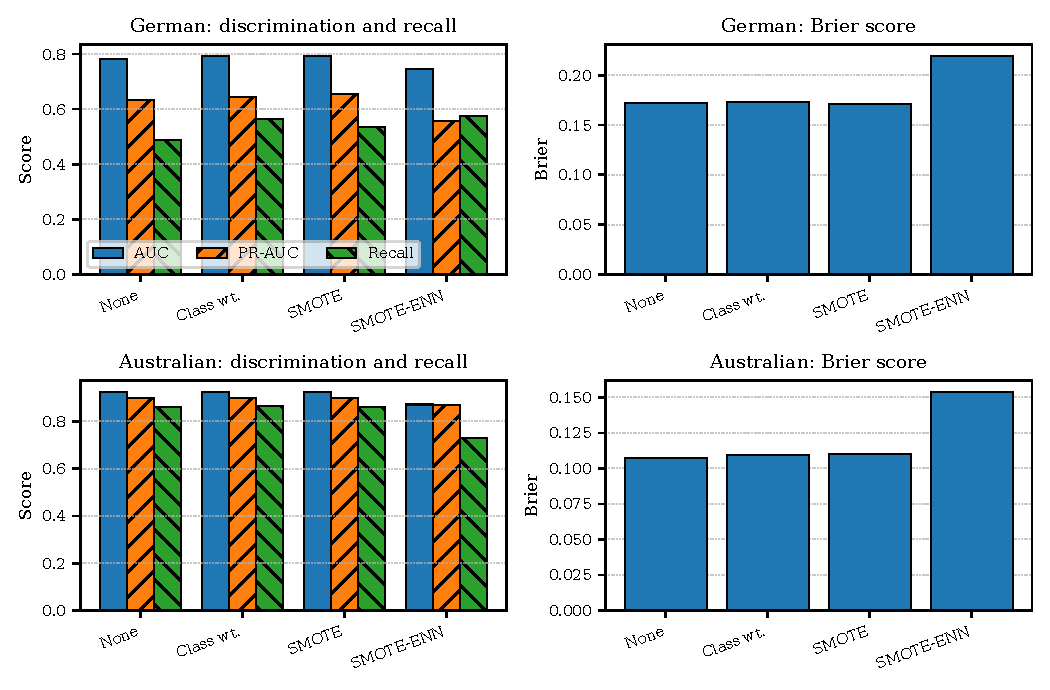
\includegraphics[width=\textwidth]{figures/fig2_imbalance.pdf}
\caption{Imbalance strategies for XGBoost under leakage-free five-fold CV
(values from Table~\ref{tab:imbalance}). SMOTE-ENN raises minority recall but
degrades AUC, PR-AUC, and calibration on both datasets; the ranking and
probability penalties are largest on German Credit. Brier score is plotted
separately because a lower value is preferable.}
\label{fig:imbalance}
\end{figure*}

\begin{table}[t]
\caption{Leakage-free five-fold CV of imbalance strategies (XGBoost).}
\label{tab:imbalance}
\centering
\footnotesize
\begin{tabular}{@{}llrrrrr@{}}
\toprule
Dataset & Strategy & AUC & PR-AUC & Recall & Prec. & Brier \\
\midrule
\multirow{4}{*}{German}
 & none        & 0.782 & 0.633 & 0.487 & 0.624 & 0.172 \\
 & class wt.\  & 0.792 & 0.643 & 0.563 & 0.608 & 0.173 \\
 & SMOTE       & 0.794 & 0.654 & 0.537 & 0.617 & 0.171 \\
 & SMOTE-ENN   & 0.746 & 0.558 & 0.577 & 0.503 & 0.220 \\
\midrule
\multirow{4}{*}{Austral.}
 & none        & 0.926 & 0.900 & 0.860 & 0.835 & 0.107 \\
 & class wt.\  & 0.924 & 0.899 & 0.866 & 0.836 & 0.109 \\
 & SMOTE       & 0.925 & 0.901 & 0.860 & 0.830 & 0.110 \\
 & SMOTE-ENN   & 0.872 & 0.868 & 0.730 & 0.821 & 0.154 \\
\bottomrule
\end{tabular}
\end{table}

\subsection{Comparison Across Boosting Families}

Table~\ref{tab:models} and Fig.~\ref{fig:models} compare six models (class
weighting for XGB, unweighted otherwise). On German data, RF attains the best
AUC (0.800) and Brier score (0.163); among the boosting families CatBoost has
the best Brier score (0.164) and a near-best AUC (0.791), while XGBoost has the
best PR-AUC (0.652). On Australian data RF leads on all three metrics
(0.936/0.923/0.100). The three boosting families differ by at most 0.023 AUC,
so family choice appears less consequential than imbalance strategy,
calibration, and explanation reliability---which motivates our focus on the
audit layer rather than on the predictor. Because XGB is class-weighted while
the others are not, and no model is tuned, this comparison is indicative only.

\begin{figure*}[t]
\centering
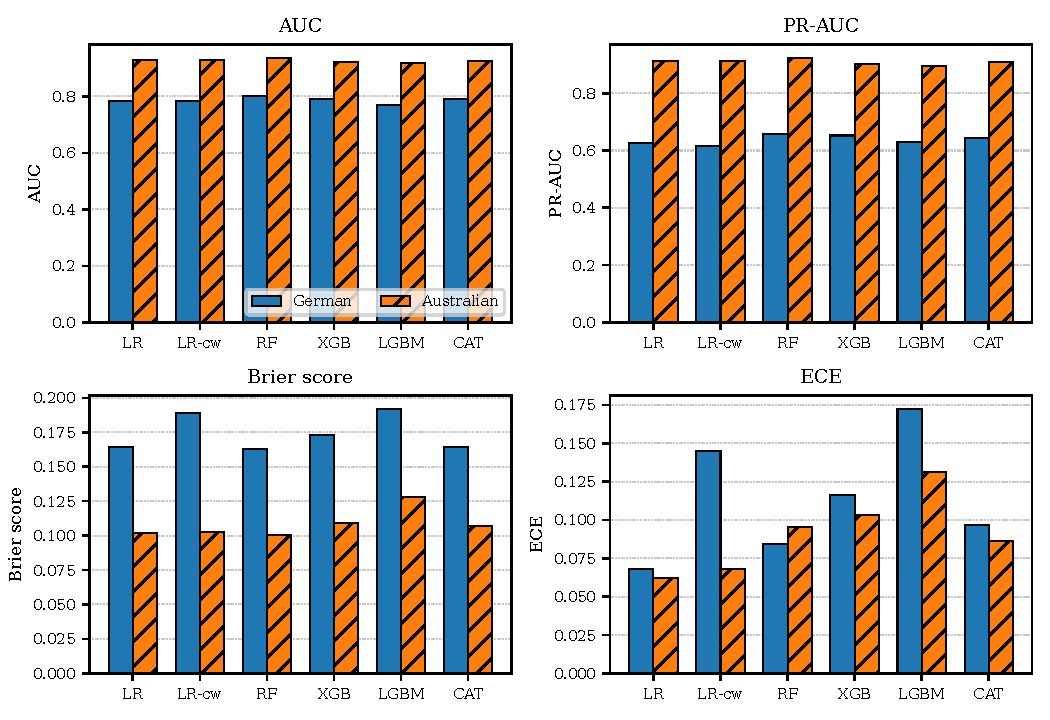
\includegraphics[width=\textwidth]{figures/fig3_models.pdf}
\caption{Model comparison on the two datasets (values from
Table~\ref{tab:models}), grouped per metric. AUC and PR-AUC are better when
higher; Brier score is better when lower. RF and CatBoost give the most
reliable probabilities among the six models, and the boosting families are
separated by margins smaller than the effect of calibration.}
\label{fig:models}
\end{figure*}

\begin{table}[t]
\caption{Model comparison, five-fold CV: AUC / PR-AUC / Brier.}
\label{tab:models}
\centering
\footnotesize
\begin{tabular}{@{}lrrrrrr@{}}
\toprule
Dataset & LR & LR-cw & RF & XGB & LGBM & CAT \\
\midrule
German AUC   & .784 & .785 & .800 & .792 & .770 & .791 \\
German PR    & .625 & .616 & .656 & .652 & .630 & .645 \\
German Brier & .164 & .189 & .163 & .173 & .192 & .164 \\
\midrule
Austral.\ AUC   & .928 & .927 & .936 & .922 & .918 & .925 \\
Austral.\ PR    & .911 & .911 & .923 & .903 & .895 & .908 \\
Austral.\ Brier & .102 & .103 & .100 & .109 & .128 & .107 \\
\bottomrule
\end{tabular}
\end{table}

\subsection{Calibration}

Table~\ref{tab:calibration} reports the single-split calibration study, and
Fig.~\ref{fig:calibration} summarises it. Isotonic regression reduces ECE from
0.136 to 0.060 on German data ($-56\%$) and from 0.106 to 0.066 on Australian
data ($-38\%$). On Australian data the Brier score improves (0.121 to 0.117)
but AUC falls (0.920 to 0.914). On German data the Brier score improves
(0.183 to 0.163) and AUC is essentially unchanged (0.775 to 0.776). Sigmoid
scaling attains an even lower held-out ECE on both datasets (0.036 German;
0.062 Australian). This is not contradictory: the calibrator is selected on
out-of-fold development Brier (ECE as tie-breaker), not on the held-out test
set, so test-set rankings may differ. Because ECE is estimated from ten bins
over 200 test cases, it is noisy, and the percentage reductions should be read
with that in mind. Calibrated probabilities are a prerequisite for the
margin-based routing of~(\ref{eq:routing}).

\begin{figure*}[t]
\centering
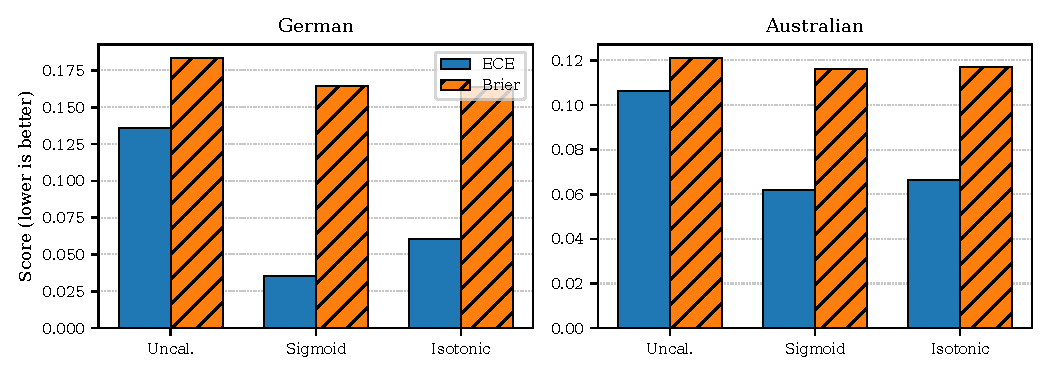
\includegraphics[width=\textwidth]{figures/fig4_calibration.pdf}
\caption{Calibration methods on both datasets (values from
Table~\ref{tab:calibration}). Isotonic regression attains the lowest held-out
expected calibration error on both datasets; sigmoid attains a lower test ECE
but is not selected by the out-of-fold Brier criterion.}
\label{fig:calibration}
\end{figure*}

\begin{table}[t]
\caption{Calibration of XGBoost (single split, held-out test set). The
calibrator is selected on out-of-fold development Brier; the selected method
is boldfaced.}
\label{tab:calibration}
\centering
\footnotesize
\begin{tabular}{@{}lrrrr@{}}
\toprule
Dataset & Method & ECE & Brier & AUC \\
\midrule
\multirow{3}{*}{German}
 & none     & 0.136 & 0.183 & 0.775 \\
 & sigmoid  & 0.036 & 0.165 & 0.775 \\
 & \textbf{isotonic} & \textbf{0.060} & \textbf{0.163} & \textbf{0.776} \\
\midrule
\multirow{3}{*}{Austral.}
 & none     & 0.106 & 0.121 & 0.920 \\
 & sigmoid  & 0.062 & 0.116 & 0.920 \\
 & \textbf{isotonic} & \textbf{0.066} & \textbf{0.117} & \textbf{0.914} \\
\bottomrule
\end{tabular}
\end{table}

\subsection{Explanation Stability and Cross-Method Agreement}

Across 150 German test cases with $K=10$ perturbations each, the mean stability
score is $\bar{S}=0.866\pm0.075$ (median 0.876), but 16.7\% of cases fall below
the $S<0.8$ review threshold (Fig.~\ref{fig:explanation}(a)); the mean
normalised attribution displacement is 0.326. Stability is nearly uncorrelated
with the decision margin ($\rho_s=0.042$): cases far from the threshold can
still carry unstable explanations. This supports the premise that margin-based
abstention alone cannot detect explanation unreliability~\cite{tufail2026signal,
marjanovic2024investigating}. On Australian data the mean is
$\bar{S}=0.870\pm0.070$ with 16.7\% of cases flagged.

The SHAP--LIME audit (100 cases, $k=5$) yields a mean top-5 Jaccard agreement
$J_5=0.353\pm0.148$ and $J_3=0.329\pm0.213$ on German Credit; on Australian
Credit it yields $J_5=0.498\pm0.183$ and $J_3=0.526\pm0.261$
(Fig.~\ref{fig:explanation}(b)). A Jaccard index of 0.353 on five-element sets
corresponds to only about two or three shared features, so two to three
top-ranked features differ between the two methods on the same case. That is a
material discrepancy for an applicant who contests a decision.

\begin{figure*}[t]
\centering
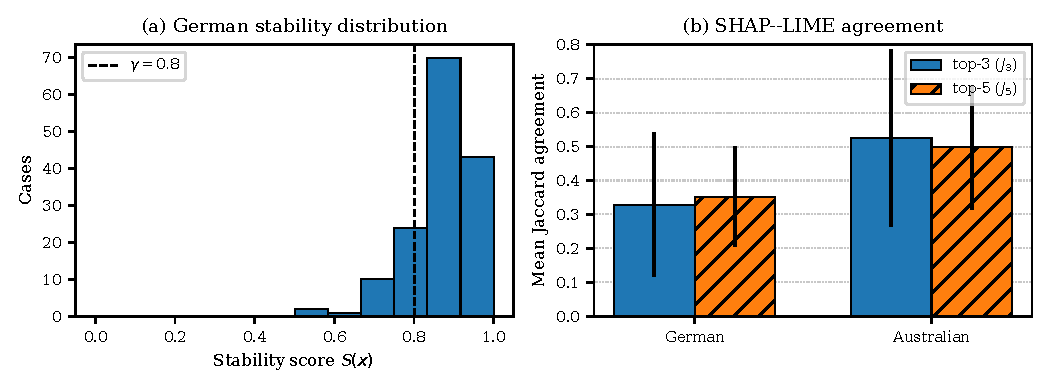
\includegraphics[width=\textwidth]{figures/fig5_explanation.pdf}
\caption{Explanation audit. (a) Distribution of per-case stability on the German
test split ($n=150$, $K=10$); the dashed line marks the $\gamma=0.8$ review
threshold. (b) Mean SHAP--LIME top-$k$ Jaccard agreement with standard deviation
on German and Australian Credit ($n=100$ per dataset).}
\label{fig:explanation}
\end{figure*}

\subsection{Reliability-Guided Routing}
\label{sec:routing}

Table~\ref{tab:routing} and Fig.~\ref{fig:routing} evaluate routing on the
German test split ($n=200$; threshold $t=0.333$). We report coverage (the
fraction decided automatically), selective error, and the composite
review-need rate $e(x)$ among auto-decided cases. Margin-only routing (P1)
reduces selective error from 0.295 to 0.182 at $\Delta=0.20$, while its
composite risk falls only from 0.385 to 0.282, because unstable explanations
persist even far from the threshold. Adding the stability rule (P2) removes
unstable-explanation cases from the automatic lane.

\begin{table}[t]
\caption{Routing on the German test split. Composite review-need
$e(x)=\mathbf{1}\{\mathrm{err}\vee S<0.8\}$; base auto-lane composite risk
0.385; base error 0.295.}
\label{tab:routing}
\centering
\footnotesize
\begin{tabular}{@{}rrrrr@{}}
\toprule
\multirow{2}{*}{$\Delta$} &
\multicolumn{2}{c}{P1: margin only} &
\multicolumn{2}{c}{P2: margin + stability} \\
\cmidrule(lr){2-3}\cmidrule(lr){4-5}
 & Cov.\ & Comp.\ & Cov.\ & Comp. \\
\midrule
0.00 & 1.000 & 0.385 & 0.875 & 0.297 \\
0.05 & 0.740 & 0.318 & 0.655 & 0.229 \\
0.10 & 0.595 & 0.311 & 0.525 & 0.219 \\
0.15 & 0.595 & 0.311 & 0.525 & 0.219 \\
0.20 & 0.550 & 0.282 & 0.490 & 0.194 \\
0.25 & 0.245 & 0.224 & 0.225 & 0.156 \\
\bottomrule
\end{tabular}
\end{table}

\emph{Matched-coverage comparison.} Policies reach different coverage at the
same $\Delta$, so we compare at equal coverage (Table~\ref{tab:matched}). At
55\% coverage P1 has composite risk 0.282 while P2 has 0.209; at 75\% the
values are 0.320 and 0.233; at 84\% they are 0.327 and 0.286. P3 is nearly
identical to P2 at every matched point. We regard matched coverage as the
fairer comparison because policies span different coverage ranges at fixed
$\Delta$.

\begin{table}[t]
\caption{Matched-coverage comparison on the German test split: composite
review-need among automatically decided cases.}
\label{tab:matched}
\centering
\footnotesize
\begin{tabular}{@{}lrrr@{}}
\toprule
Target coverage & P1 margin & P2 margin $+$ stab. & P3 $+$ conformal \\
\midrule
55\% & 0.282 & 0.209 & 0.218 \\
75\% & 0.320 & 0.233 & 0.233 \\
84\% & 0.327 & 0.286 & 0.286 \\
\bottomrule
\end{tabular}
\end{table}

\begin{figure*}[t]
\centering
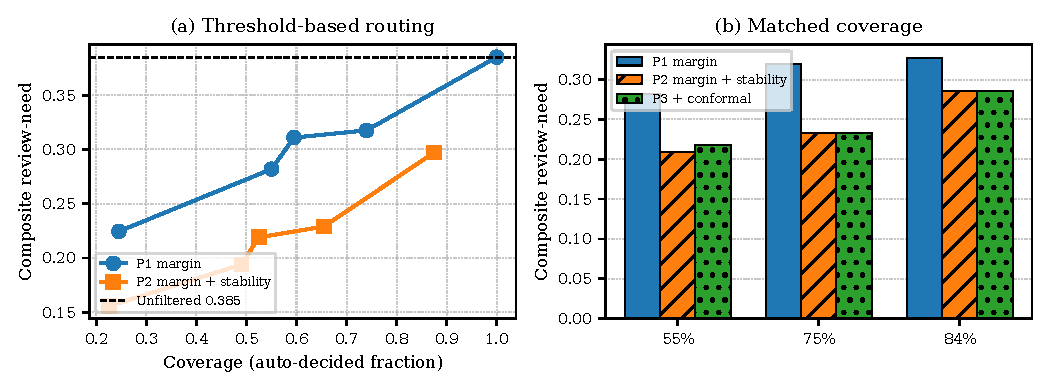
\includegraphics[width=\textwidth]{figures/fig6_routing.pdf}
\caption{Routing performance on the German test split (values from
Tables~\ref{tab:routing} and~\ref{tab:matched}). (a) Composite review-need rate
against coverage for margin-only (P1) and stability-augmented (P2) policies;
the dotted line marks the unfiltered risk of 0.385. (b) Matched-coverage
comparison at 55\%, 75\%, and 84\% coverage.}
\label{fig:routing}
\end{figure*}

\emph{Limits of the review-budget view.} We deliberately do not report a fixed
review-budget queue-precision claim: every stability-flagged case belongs to
the composite criterion by definition, so such a result would be largely true
by construction and should be read as an upper bound, not as independent
evidence of benefit. It does not establish that low $S$ identifies cases whose
explanations are harmful. What the data do show is that the two signals
identify different failure modes: stability-flagged cases are not more
error-prone (error 0.280 flagged versus 0.297 unflagged), so a policy using
only the margin or only stability misses the other failure mode. The conformal
rule with $\alpha=0.2$ fires rarely on German data, so P3 $\approx$ P2 here. We
therefore make no claim of benefit from the conformal term on these datasets;
it is expected to matter under dataset shift~\cite{angelopoulos2023conformal},
which we do not test.

\subsection{Group-Level Behaviour and Computational Overhead}

Table~\ref{tab:groups} reports group behaviour on the German test split (139
male, 61 female applicants). Female applicants exhibit higher recall (0.800
versus 0.625), a higher false-positive rate (0.415 versus 0.232), and a higher
positive-decision rate (0.541 versus 0.345). With only 61 female applicants
these estimates carry wide uncertainty. At a fixed margin threshold
$\Delta=0.20$, adding the stability condition raises review load from 45\% to
51\%, so group-specific monitoring of the auto/review split is advisable. We
further note that the model uses sex as an input feature, which is restricted
or prohibited in credit decisions in many jurisdictions; it is retained here
only to reproduce the standard benchmark, and a run without protected
attributes is required before any deployment claim. A full
fairness--accuracy--stability Pareto analysis is left to future
work~\cite{das2023algorithmic}.

\begin{table}[t]
\caption{Group behaviour on the German test split under the calibrated model
and the P2 routing rule.}
\label{tab:groups}
\centering
\footnotesize
\begin{tabular}{@{}lrrrrrr@{}}
\toprule
Group & $n$ & Recall & FPR & Pos.\ dec.\ & Auto dec.\ & Review \\
\midrule
Female & 61  & 0.800 & 0.415 & 0.541 & 0.443 & 0.557 \\
Male   & 139 & 0.625 & 0.232 & 0.345 & 0.511 & 0.489 \\
\bottomrule
\end{tabular}
\end{table}

\emph{Overhead.} Table~\ref{tab:overhead} reports measured latency. Prediction
is fast (about 0.15~ms/case). The stability audit ($K=10$ TreeSHAP calls) adds
32.1~ms/case on German and 39.2~ms/case on Australian data; the SHAP--LIME
audit costs 445.1~ms/case and 279.4~ms/case, respectively. CatBoost training is
approximately 1.3--1.4$\times$ XGBoost training on these datasets. The
explanation audit is therefore a batch-time cost of hundreds of milliseconds
per case, not a few milliseconds of online latency; any deployment would need
to precompute or amortise it.

\begin{table}[t]
\caption{Measured audit overhead (ms per case).}
\label{tab:overhead}
\centering
\footnotesize
\begin{tabular}{@{}lrrr@{}}
\toprule
Dataset & Prediction & Stability ($K=10$) & SHAP--LIME \\
\midrule
German     & 0.15 & 32.1 & 445.1 \\
Australian & 0.15 & 39.2 & 279.4 \\
\bottomrule
\end{tabular}
\end{table}

\section{Threats to Validity}
\label{sec:threats}

\emph{Internal.} Results use fixed seed 42, and the routing analysis relies on
a single 80/20 split. Stability scores are computed for a 150-case subsample,
and the remaining 50 test cases are assigned the median score, which can never
trigger the $S<0.8$ rule; this understates P2's flagged share and may distort
its composite risk. The composite metric shares the stability condition with
P2, as discussed in Section~\ref{sec:routing}. Four extensions are
\emph{planned}, not executed, and are therefore reported as future work rather
than as results: (i) a sensitivity sweep of $S(x)$ and the prediction-flip rate
over perturbation half-widths of 1\%, 2.5\%, 5\%, and 10\%; (ii) a breakdown of
$S$ and $J_5$ by imbalance strategy and boosting family, which would test the
qualitative claim of~\cite{tufail2026signal}; (iii) repetition of the
calibration, stability, and routing analyses on a larger credit dataset such
as the Taiwan default-of-credit-card-clients data~\cite{yeh2009comparisons};
and (iv) fixed-review-budget and cost-sensitive evaluations.

\emph{External.} Two public datasets with 20 and 14 attributes may not transfer
to high-cardinality bureau data. The German cost matrix (5:1) is not modelled,
and asymmetric costs would change the optimal threshold and routing policy.
Ordinal encoding of nominal attributes means SMOTE may interpolate between
unordered categories; SMOTE-NC or one-hot encoding~\cite{chawla2002smote} is
preferable.

\emph{Construct.} $S(x)$ measures rank stability of attributions, not
faithfulness; SHAP--LIME disagreement partially covers this, but faithfulness
metrics should complement it.

\section{Conclusion}
\label{sec:conclusion}

We presented a stability-aware, confidence-guided audit layer for credit risk
models that combines leakage-free imbalance handling, probability calibration,
per-case explanation stability under plausibility-preserving perturbations, a
SHAP--LIME agreement audit, and a human-review routing rule. On German and
Australian credit data: (i) the recall gains of SMOTE-ENN come at a material
cost to ranking and calibration; (ii) isotonic calibration reduces ECE by up to
56\%, with a small AUC change that is near-zero on German and negative on
Australian data; (iii) 16.7\% of German test cases carry explanation
instability that the decision margin does not reveal ($\rho_s=0.042$); and
(iv) at 55\% coverage, adding the stability rule lowers composite auto-lane
risk from 0.282 to 0.209, a gain that is partly definitional. The main lesson
is that margin-based and explanation-based reliability are complementary
failure modes. Future work includes external validation of $S(x)$ against
human or counterfactual criteria, cost-sensitive thresholds, richer
perturbation models, tests under dataset shift where the conformal term should
matter, and conformal guarantees conditional on group membership.

\section*{Reproducibility}
All experiments use fixed seeds (42). The pipeline requires Python 3.13.5 with
NumPy 2.1.3, pandas 2.2.3, SciPy 1.15.3, scikit-learn 1.6.1,
imbalanced-learn 0.13.0, XGBoost 3.4.1, LightGBM 4.7.0, CatBoost 1.2.10,
SHAP 0.54.1, and LIME 0.2.0.1. The audit defaults are 150 stability cases,
10 perturbations, 100 SHAP--LIME cases, 1500 LIME samples, and predicted-label
conformal scoring. Code, per-case result files, and figure-generation scripts
accompany the submission.

\begin{thebibliography}{99}

\bibitem{chawla2002smote}
N.~V. Chawla, K.~W. Bowyer, L.~O. Hall, and W.~P. Kegelmeyer, ``SMOTE:
synthetic minority over-sampling technique,'' \emph{J. Artif. Intell. Res.},
vol.~16, pp.~321--357, 2002.

\bibitem{batista2004study}
G.~E.~A.~P.~A. Batista, R.~C. Prati, and M.~C. Monard, ``A study of the behavior
of several methods for balancing machine learning training data,''
\emph{ACM SIGKDD Explor. Newsl.}, vol.~6, no.~1, pp.~20--29, 2004.

\bibitem{guo2017calibration}
C.~Guo, G.~Pleiss, Y.~Sun, and K.~Q. Weinberger, ``On calibration of modern
neural networks,'' in \emph{Proc. ICML}, 2017, pp.~1321--1330.

\bibitem{lundberg2017unified}
S.~M. Lundberg and S.-I. Lee, ``A unified approach to interpreting model
predictions,'' in \emph{Proc. NeurIPS}, vol.~30, 2017.

\bibitem{ribeiro2016why}
M.~T. Ribeiro, S.~Singh, and C.~Guestrin, ```Why should I trust you?':
Explaining the predictions of any classifier,'' in \emph{Proc. ACM SIGKDD},
2016, pp.~1135--1144.

\bibitem{alvarezmelis2018robustness}
D.~Alvarez-Melis and T.~S.~Jaakkola, ``On the robustness of interpretability
methods,'' \emph{arXiv:1806.08049}, 2018.

\bibitem{ghorbani2019interpretation}
A.~Ghorbani, A.~Abid, and J.~Zou, ``Interpretation of neural networks is
fragile,'' in \emph{Proc. AAAI}, vol.~33, 2019, pp.~3681--3688.

\bibitem{krishna2022disagreement}
S.~Krishna \emph{et al.}, ``The disagreement problem in explainable machine
learning: A practitioner's perspective,'' \emph{arXiv:2202.01602}, 2022.

\bibitem{aruleba2024credit}
I.~Aruleba and Y.~Sun, ``Effective credit risk prediction using ensemble
classifiers with model explanation,'' \emph{IEEE Access}, vol.~12,
pp.~115015--115025, 2024.

\bibitem{aruleba2025improved}
I.~Aruleba and Y.~Sun, ``An improved ensemble method with data resampling for
credit risk prediction,'' \emph{IEEE Access}, vol.~13, pp.~71275--71287, 2025.

\bibitem{nguyen2025comparative}
N.~Nguyen and D.~Ngo, ``Comparative analysis of boosting algorithms for
predicting personal default,'' \emph{Cogent Econ. Finance}, vol.~13, no.~1,
p.~2465971, 2025.

\bibitem{kwon2026generative}
T.~Kwon, ``Generative deep learning for class imbalance in credit risk
modeling: Comparative evaluation of synthetic oversampling methods and an
elastic oversampling extension,'' \emph{Financial Innovation}, vol.~12, no.~1,
p.~161, 2026.

\bibitem{chab2026csanet}
T.~Chab and J.~Jeon, ``CSA-Net: A type-aware dual-tower neural model for
imbalanced tabular credit default prediction,'' \emph{IEEE Access}, vol.~14,
2026.

\bibitem{shawabkeh2026explainable}
Y.~T. Shawabkeh, A.~A.~B.~Atta, K.~A.~Aldarabah, and R.~Alofishat,
``Explainable machine learning models for AI enabled credit scoring and
financial inclusion in emerging markets,'' \emph{Discover Artif. Intell.},
vol.~6, p.~1418, 2026.

\bibitem{japinye2025explainable}
A.~O. Japinye and A.~A.~Adedugbe, ``Explainable AI for credit scoring with
SHAP-calibrated ensembles: A multi-market evaluation on public lending data,''
\emph{Risks}, vol.~13, no.~3, p.~45, 2025.

\bibitem{tufail2026signal}
A.~Tufail and M.~K.~Sohail, ``From signal to noise: How class imbalance erodes
trust in credit-scoring explanations,'' \emph{J. Innov. Res. Manag. Sci.},
pp.~26--51, 2026.

\bibitem{he2009learning}
H.~He and E.~A. Garcia, ``Learning from imbalanced data,'' \emph{IEEE Trans.
Knowl. Data Eng.}, vol.~21, no.~9, pp.~1263--1284, 2009.

\bibitem{lundberg2020local}
S.~M. Lundberg \emph{et al.}, ``From local explanations to global
understanding with explainable AI for trees,'' \emph{Nat. Mach. Intell.},
vol.~2, no.~1, pp.~56--67, 2020.

\bibitem{misheva2021explainable}
B.~H. Misheva \emph{et al.}, ``Explainable artificial intelligence in credit
risk management,'' \emph{arXiv:2103.00949}, 2021.

\bibitem{xin2026explainable}
Q.~Xin, ``Explainable and fair credit risk scoring with counterfactual
explanations: A reproducible evaluation on the German credit dataset,''
\emph{J-INTECH}, 2026.

\bibitem{platt1999probabilistic}
J.~Platt, ``Probabilistic outputs for support vector machines and comparisons
to regularized likelihood methods,'' in \emph{Advances in Large Margin
Classifiers}. MIT Press, 1999, pp.~61--74.

\bibitem{zadrozny2002transforming}
B.~Zadrozny and C.~Elkan, ``Transforming classifier scores into accurate
multiclass probability estimates,'' in \emph{Proc. ACM SIGKDD}, 2002,
pp.~694--699.

\bibitem{niculescu2005predicting}
A.~Niculescu-Mizil and R.~Caruana, ``Predicting good probabilities with
supervised learning,'' in \emph{Proc. ICML}, 2005, pp.~625--632.

\bibitem{geifman2017selective}
Y.~Geifman and R.~El-Yaniv, ``Selective classification for deep neural
networks,'' in \emph{Proc. NeurIPS}, vol.~30, 2017.

\bibitem{angelopoulos2023conformal}
A.~N. Angelopoulos and S.~Bates, ``Conformal prediction: A gentle
introduction,'' \emph{Found. Trends Mach. Learn.}, vol.~16, no.~4,
pp.~494--591, 2023.

\bibitem{vovk2005algorithmic}
V.~Vovk, A.~Gammerman, and G.~Shafer, \emph{Algorithmic Learning in a Random
World}. Springer, 2005.

\bibitem{marjanovic2024investigating}
S.~V. Marjanovi\'c, I.~Augenstein, and C.~Lioma, ``Investigating the impact of
model instability on explanations and uncertainty,'' in \emph{Findings of
ACL}, 2024.

\bibitem{youden1950index}
W.~J. Youden, ``Index for rating diagnostic tests,'' \emph{Cancer}, vol.~3,
no.~1, pp.~32--35, 1950.

\bibitem{hofmann1994statlog}
H.~Hofmann, ``Statlog (German credit data),'' UCI Machine Learning Repository,
1994.

\bibitem{quinlan1987statlog}
R.~Quinlan, ``Statlog (Australian credit approval),'' UCI Machine Learning
Repository, 1987.

\bibitem{yeh2009comparisons}
I.-C. Yeh and C.~Lien, ``The comparisons of data mining techniques for the
predictive accuracy of probability of default of credit card clients,''
\emph{Expert Syst. Appl.}, vol.~36, no.~2, pp.~2473--2480, 2009.

\bibitem{breiman2001random}
L.~Breiman, ``Random forests,'' \emph{Mach. Learn.}, vol.~45, no.~1,
pp.~5--32, 2001.

\bibitem{chen2016xgboost}
T.~Chen and C.~Guestrin, ``XGBoost: A scalable tree boosting system,'' in
\emph{Proc. ACM SIGKDD}, 2016, pp.~785--794.

\bibitem{ke2017lightgbm}
G.~Ke \emph{et al.}, ``LightGBM: A highly efficient gradient boosting decision
tree,'' in \emph{Proc. NeurIPS}, vol.~30, 2017.

\bibitem{prokhorenkova2018catboost}
L.~Prokhorenkova, G.~Gusev, A.~Vorobev, A.~V.~Dorogush, and A.~Gulin,
``CatBoost: Unbiased boosting with categorical features,'' in \emph{Proc.
NeurIPS}, vol.~31, 2018, pp.~6639--6649.

\bibitem{das2023algorithmic}
S.~Das, R.~Stanton, and N.~Wallace, ``Algorithmic fairness,'' \emph{Annu. Rev.
Financial Econ.}, 2023.

\end{thebibliography}

\end{document}
